\documentclass[11pt]{article}
\title{\textbf{Triple unit}}
\author{https://github.com/heptagons/meccano/units/triple}
\date{}

\usepackage{../../meccano}
\usepackage{tikz}
\usetikzlibrary{calc}

\begin{document}

\maketitle
\begin{abstract}
A \textbf{Triple unit} is a group of \textbf{five} meccano\meccanoref strips $a,b,c,d,e$
forming \textbf{three equal angles} $\theta$ intended to build three consecutive perimeter sides
of some regular polygons.
We look for integer values of strip $e$ in function of integer values of sides $a,b,c,d$ and 
a particular angle $\theta$.
We confirm a generic equation found matches the one used to build pentagons of type 2 \footnote{
\href{https://github.com/heptagons/meccano/blob/main/penta/pentagons.pdf}{Meccano pentagons}}.
Here we found a lot of hexagons and filter some not trivial solutions.
We look for octagons, decagons and dodecagons.
\end{abstract}.

\begin{figure}[h]
\centering
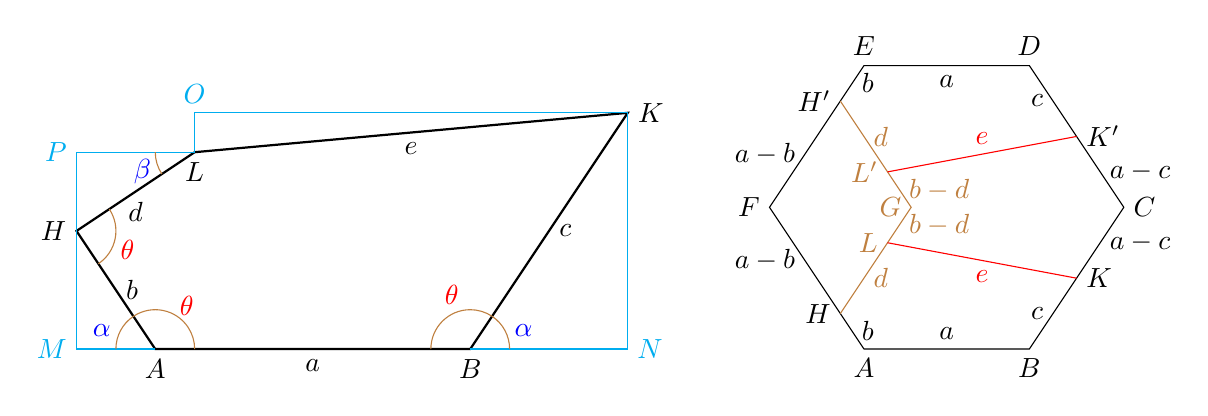
\begin{tikzpicture}
\begin{scope}[scale=0.5] %left figure
\draw[black,thick] (0,0)
-- node[below] {$a$} ++(8,0) node[below]{$B$}
-- node[below,right] {$c$} ++(4,6) node[right]{$K$}
-- node[below] {$e$} ++(-11,-1) node[right,below]{$L$}
-- node[below] {$d$} ++(-3,-2) node[left]{$H$}
-- node[right] {$b$} cycle node[below]{$A$};
\draw[cyan] (0,0)
-- ++(-2,0) node[below,left] {$M$}
-- ++(0,3)
-- ++(0,2) node[above,left] {$P$}
-- ++(3,0)
-- ++(0,1) node[above] {$O$}
-- ++(11,0);
\draw[cyan] (8,0)
-- ++(4,0) node[below,right] {$N$}
-- ++(0,6);
\draw[brown] (0,0)+(-1,0)
 arc(180:180-atan(3/2):1) node[midway,above,left,blue] {$\alpha$}
 arc(180-atan(3/2):0:1) node[above,red,pos=0.7] {$\theta$};
\draw[brown] (8,0)+(-1,0)
 arc(180:atan(3/2):1) node[above,red,pos=0.5] {$\theta$}
 arc(atan(3/2):0:1) node[midway,above,right,blue] {$\alpha$};
\draw[brown] (-2,3)+(0.832,0.554) %sin(atan(3/2),cos(atan(3/2))
 arc(atan(2/3):-atan(3/2):1) node[right,red,pos=0.7] {$\theta$};
\draw[brown] (1,5)+(-0.832,-0.554)
 arc(180+atan(2/3):180:1) node[left,blue,pos=0.1] {$\beta$};
\end{scope}

\begin{scope}[scale=0.30,shift={(30,0)}]
\draw[black](0,0)
 -- node[above] {$a$} ++(7,0) node[below]{$B$}
 -- node[left] {$c$} ++(2,3) node[right]{$K$}
 -- node[right] {$a-c$} ++(2,3) node[right]{$C$}
 -- node[right] {$a-c$} ++(-2,3) node[right]{$K'$}
 -- node[left] {$c$} ++(-2,3) node[above]{$D$}
 -- node[below] {$a$} ++(-7,0) node[above]{$E$}
 -- node[right] {$b$} ++(-1,-1.5) node[left]{$H'$}
 -- node[left] {$a-b$} ++(-3,-4.5) node[left]{$F$}
 -- node[left] {$a-b$} ++(+3,-4.5) node[left]{$H$}
 -- node[right] {$b$} ++(1,-1.5) node[below]{$A$};
\draw[brown](-1,1.5)
 -- node[above,right]{$d$} ++(2,3) node[left]{$L$}
 -- node[right]{$b-d$} ++(1,1.5) node[left]{$G$}
 -- node[right]{$b-d$} ++(-1,1.5) node[left]{$L'$}
 -- node[below,right]{$d$} ++(-2,3) node[]{};
\draw[red](1,4.5) -- node[below]{$e$} ++(8,-1.5);
\draw[red](1,7.5) -- node[above]{$e$} ++(8,1.5);
\end{scope}

\end{tikzpicture}
\caption{
At the left we have the Triple unit (three angles $\theta$) with the strips $a,b,c,d,e$.
At the right we use two units to build a regular polygon of side $a$ extending strips $b,c,d$ to fix everthing. This construction is possible only when $a > b,c$.
}
\label{fig:triple}
\end{figure}

\section{Algebra}

From nodes $A$ and $B$ of fig \ref{fig:triple} we get $\alpha$ from $\theta$ ($\pi = 180^\circ$):
\begin{align}
\theta &= \pi - \alpha \nonumber\\
\alpha &= \pi - \theta
\end{align}
And from node $H$ we get $\beta$ from $\theta$:
\begin{align}
\theta &= \alpha + \beta \nonumber\\
\beta &= \theta - \alpha = \theta - (\pi - \theta) = 2\theta - \pi
\end{align}

We calculate horizontal segment $\overline{OK}$:
\begin{align}
\overline{OK} &= \overline{MA} + a + \overline{BN} - \overline{PL} \nonumber\\
 &= b\cos{\alpha} + a + c\cos{\alpha} - d\cos{\beta} \nonumber\\
 &= a + (b+c)\cos{\alpha} - d\cos{\beta} \nonumber\\
 &= a + (b+c)\cos{(\pi-\theta)} - d\cos{(2\theta - \pi)} \nonumber\\
 &= a - (b+c)\cos{\theta} + d\cos{(2\theta)}
\end{align} 

And vertical segment $\overline{OL}$:
\begin{align}
\overline{OL} &= \overline{KN} - \overline{PH} - \overline{HM} \nonumber\\
 &= c\sin{\alpha} - d\sin{\beta} - b\sin{\alpha} \nonumber\\
 &= (c-b)\sin{\alpha} - d\sin{\beta} \nonumber\\
 &= (c-b)\sin{(\pi-\theta)} - d\sin{(2\theta-\pi)} \nonumber\\
 &= (c-b)\sin{\theta} + d\sin{(2\theta)}
\end{align}

So we can express $e$ in function of $a,b,c,d$ and angle $\theta$:
\begin{align}
e^2 &= (\overline{OK})^2 + (\overline{OL})^2 \nonumber\\
 &= (a -(b+c)\cos\theta +d\cos(2\theta))^2 +((c-b)\sin\theta +d\sin(2\theta))^2 \nonumber\\
 &= a^2 +(b^2+2bc+c^2)\cos^2\theta + d^2\cos^2(2\theta) + (c^2-2cb+b^2)sin^2\theta +d^2\sin^2(2\theta) \nonumber\\
 &\qquad -2a(b+c)\cos\theta +2ad\cos(2\theta) -2(b+c)d\cos\theta\cos(2\theta) \nonumber\\
 &\qquad +2(c-b)d\sin\theta\sin(2\theta) \nonumber\\
%
 &= a^2 +b^2 +c^2 +d^2 +2bc\cos^2\theta -2bc\sin^2\theta \nonumber\\
 &\qquad -2a(b+c)\cos\theta +2ad\cos(2\theta) \nonumber\\
 &\qquad -2d((b+c)\cos\theta\cos(2\theta) + (b-c)\sin\theta\sin(2\theta)) \\
%
 &= a^2 +b^2 +c^2 +d^2 +2bc(\cos^2\theta -\sin^2\theta) 
  -2a(b+c)\cos\theta +2ad\cos(2\theta) \nonumber\\
 &\qquad -2d(b(\cos\theta\cos(2\theta)+\sin\theta\sin(2\theta)) 
  + c(\cos\theta\cos(2\theta)-\sin\theta\sin(2\theta))) \nonumber\\
%  
 &= a^2 +b^2 +c^2 +d^2 +2bc\cos(2\theta) 
  -2a(b+c)\cos\theta +2ad\cos(2\theta) \nonumber\\
 &\qquad -2d(b\cos(\theta-2\theta) + c\cos(\theta+2\theta)) \nonumber\\
% 
 &= a^2 +b^2 +c^2 +d^2 +2(bc+ad)\cos(2\theta) -2a(b+c)\cos\theta -2d(b\cos\theta + c\cos(3\theta)) \nonumber\\
% 
 &= a^2 +b^2 +c^2 +d^2 +2(bc+ad)\cos(2\theta) -2(ab+ac)\cos\theta -2(bd\cos\theta + cd\cos(3\theta)) \end{align}

\boxedeq{eq:triple}{
 e^2 = a^2 +b^2 +c^2 +d^2 -2(ab+ac+bd)\cos\theta +2(bc+ad)\cos(2\theta) -2cd\cos(3\theta)
}

\section{Regular polygons}

\begin{table}[h]
\centering
\begin{tabular}{|c c c c c c|}\hline
Polygon & $\theta$ & $\cos\theta$ & $\cos(2\theta)$ & $\cos(3\theta)$ & Notes 
 \rule[-2ex]{0pt}{6ex}\\ \hline\hline 
Pentagon & $\dfrac{3\pi}{5}$ &
 $\dfrac{1-\sqrt{5}}{4}$ & $\dfrac{-1-\sqrt{5}}{4}$ & $\dfrac{1+\sqrt{5}}{4}$ & 
 \rule[-2ex]{0pt}{6ex}\\ \hline
Hexagon & $\dfrac{2\pi}{3}$ &
 $-\dfrac{1}{2}$ & $-\dfrac{1}{2}$ & $1$ & 
 \rule[-2ex]{0pt}{6ex}\\ \hline
Heptagon & $\dfrac{5\pi}{7}$ &
 $-\cos{B}$ & $\cos{C}$ & $\cos{A}$ & $\cos{A}\cos{B}\cos{C} = -\frac{1}{8} $
 \rule[-2ex]{0pt}{6ex}\\ \hline
Octagon & $\dfrac{3\pi}{4}$ &
 $-\dfrac{\sqrt{2}}{2}$ & $0$ & $\dfrac{\sqrt{2}}{2}$ & 
 \rule[-2ex]{0pt}{6ex}\\ \hline
Decagon & $\dfrac{4\pi}{5}$ &
 $\dfrac{-1-\sqrt{5}}{4}$ & $\dfrac{-1+\sqrt{5}}{4}$ & $\dfrac{-1+\sqrt{5}}{4}$ &
 \rule[-2ex]{0pt}{6ex}\\ \hline
Dodecagon & $\dfrac{5\pi}{6}$ &
 $-\dfrac{\sqrt{3}}{2}$ &  &  &
 \rule[-2ex]{0pt}{6ex}\\ \hline

\end{tabular}
\caption{Regular polygons internal angles and cosines.}
\label{tbl:polygons}
\end{table}

We will test last equation into several polygons. Table \ref{tbl:polygons}
show the possible constructions and the angles and cosines.
Only when we'll get $e$ integer we'll have a solution.

\section{Equilateral pentagons}

We replace the cosines for pentagon in table \ref{tbl:polygons} in equation \ref{eq:triple}:
\begin{align}
e^2 &= a^2 +b^2 +c^2 +d^2 -2(ab+ac+bd)\cos\theta +2(bc+ad)\cos(2\theta) -2cd\cos(3\theta) \nonumber\\
 &= a^2 +b^2 +c^2 +d^2
  -2(ab+ac+bd)\left(\dfrac{1-\sqrt{5}}{4}\right)
  +2(bc+ad)\left(\dfrac{-1-\sqrt{5}}{4}\right)
  -2cd\left(\dfrac{1+\sqrt{5}}{4}\right) \nonumber\\
 &= a^2 +b^2 +c^2 +d^2 -\frac{ab+ac+bd+bc+ad+cd}{2} +\frac{ab+ac+bd-bc-ad-cd}{2}\sqrt{5}
\end{align}
$e$ cannot to be and integer if the factor of $\sqrt{5}$ is not zero so we force this factor to be zero:
\begin{align}
 ab+ac+bd-bc-ad-cd &= 0\nonumber\\
 ab+ac+bd &= bc+ad+cd \\
 ab+ac-bc &= (a-b+c)d
\end{align}
We replace $ab+ac+bd$ by $bc+ad+cd$ in the $e^2$ equation to get:
\begin{align}
e^2 &= a^2 +b^2 +c^2 +d^2 -\frac{(bc+ad+cd)+bc+ad+cd}{2} +\frac{0}{2}\sqrt{5} \nonumber\\
 &= a^2 +b^2 +c^2 +d^2 -bc -ad -cd
\end{align}

\coloredeq{eq:pentagon-e}{
e = \sqrt{a^2 +b^2 +c^2 +d^2 -bc -(a+c)d } \quad\Longleftrightarrow\quad ab+ac-bc = (a-b+c)d
}

The last formula matches the formula used in the paper Meccano pentagons which finds several pentagons of type 2. 


\section{Equilateral hexagons}

We replace the cosines for hexagon in table \ref{tbl:polygons} in equation \ref{eq:triple}:
\begin{align}
e^2 &= a^2 +b^2 +c^2 +d^2 -2(ab+ac+bd)\cos\theta +2(bc+ad)\cos(2\theta) -2cd\cos(3\theta) \nonumber\\
 &= a^2 +b^2 +c^2 +d^2 -2(ab+ac+bd)\left(-\frac{1}{2}\right) +2(bc+ad)\left(-\frac{1}{2}\right) -2cd(1) \nonumber\\
 &= a^2 +b^2 +c^2 +d^2 +ab+ac+bd -bc-ad-2cd \nonumber\\
 &= (a+b)^2 +(c-d)^2 -ab+ac+bd-bc-ad\nonumber\\
 &= (a+b)^2 +(c-d)^2 +(c-d)(a-b) -ab \nonumber\\
 &= (a+b)^2 +(c-d)(a-b+c-d) -ab
\end{align} 

\coloredeq{eq:hexagon-e}{
e &= \sqrt{(a+b)^2 +(c-d)(a-b+c-d) -ab}
}

\subsection{Hexagons software}
We wrote software code to look for hexagons using the formula for $e$ and set several
filters to prevent trivial solutions. We say an hexagon is nice when $e \leq a$.
Next is a partial list of nice hexagons:
\begin{lstlisting}
  1  a=  7 b=  1 c=  2 d=  6 e=  7
  2  a=  7 b=  1 c=  4 d=  6 e=  7
  3  a= 13 b=  2 c=  5 d= 11 e= 13
  4  a= 13 b=  2 c=  6 d= 11 e= 13
  5  a= 14 b=  1 c=  6 d= 13 e= 13
  6  a= 14 b=  1 c=  7 d= 13 e= 13
  7  a= 15 b=  1 c=  5 d= 14 e= 14
  8  a= 15 b=  1 c=  9 d= 14 e= 14
  9  a= 19 b=  2 c=  3 d= 17 e= 19
 10  a= 19 b=  2 c= 14 d= 17 e= 19
 11  a= 20 b=  1 c=  4 d= 19 e= 19
 12  a= 20 b=  1 c= 15 d= 19 e= 19
     ...
105  a= 58 b=  5 c= 10 d= 53 e= 57
106  a= 58 b=  5 c= 43 d= 53 e= 57
107  a= 59 b=  1 c= 27 d= 58 e= 52
108  a= 59 b=  1 c= 31 d= 58 e= 52
109  a= 59 b=  4 c= 11 d= 55 e= 57
110  a= 59 b=  4 c= 44 d= 55 e= 57
111  a= 59 b=  5 c= 19 d= 54 e= 56
112  a= 59 b=  5 c= 35 d= 54 e= 56
--- PASS: TestHexagonsNice (0.01s)
\end{lstlisting}
Results from \texttt{github.com/heptagons/meccano/units/triple/triple\_test.go TestHexagonsNice}

\subsection{Hexagons examples}

\begin{figure}[h]
\centering
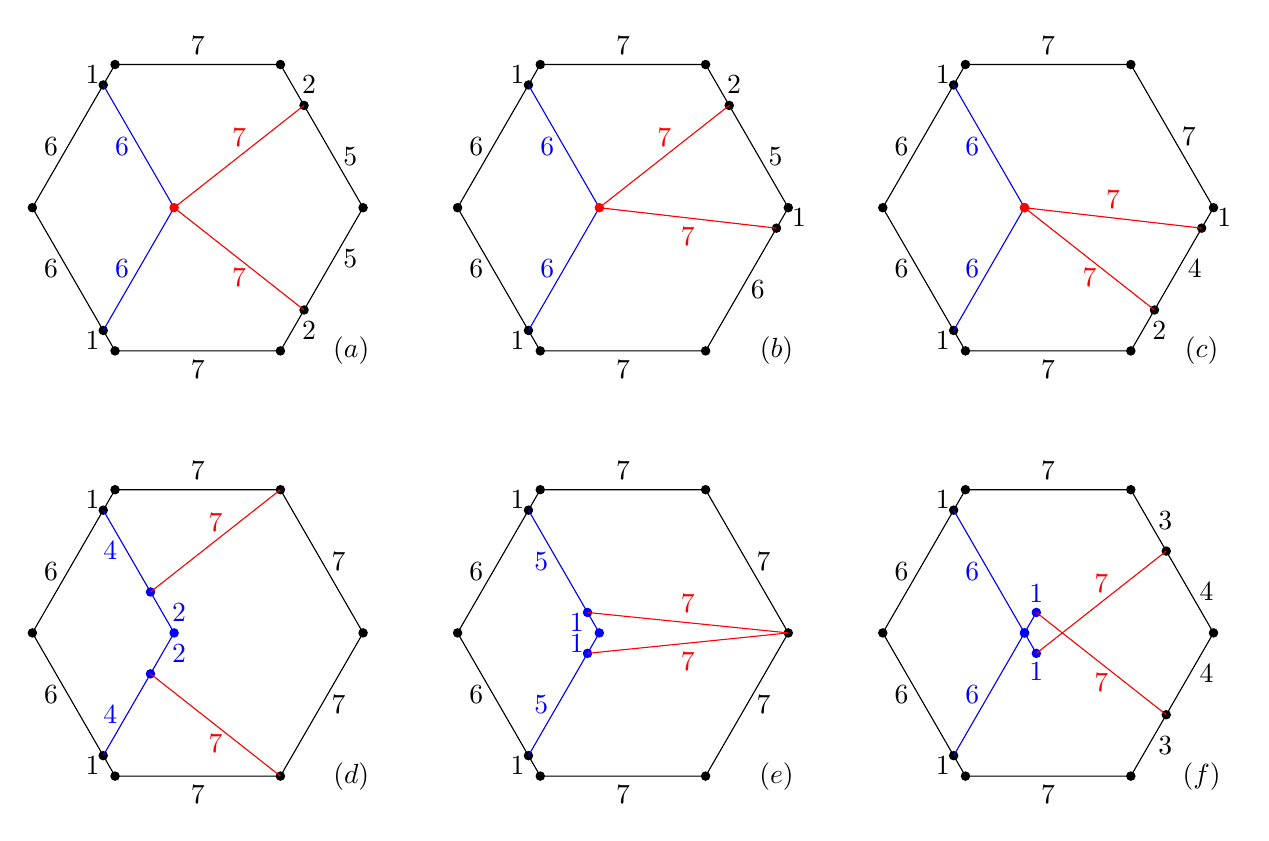
\begin{tikzpicture}
\def\x{0.5}
\def\y{0.866}
\begin{scope}[scale=0.3]

\begin{scope}[shift={(0,0)}] %row-1 col-2
\draw[black](10,0) node{$(a)$};
\draw[black,fill=black](0,0)
 -- node[below] {7} ++(7,0) circle(5pt)
 -- node[right] {2} ++(2*\x,2*\y) circle(5pt)
 -- node[right] {5} ++(5*\x,5*\y) circle(5pt)
 -- node[right] {5} ++(-5*\x,5*\y) circle(5pt)
 -- node[right] {2} ++(-2*\x,2*\y) circle(5pt)
 -- node[above] {7} ++(-7,0) circle(5pt)
 -- node[left] {1} ++(-\x,-\y) circle(5pt)
 -- node[left] {6} ++(-6*\x,-6*\y) circle(5pt)
 -- node[left] {6} ++(+6*\x,-6*\y) circle(5pt)
 -- node[left] {1} ++(\x, -\y) circle(5pt);
\draw[blue] (-1*\x,+1*\y) -- node[left] {6} ++(6*\x,6*\y);
\draw[blue] (5*\x,7*\y) -- node[left] {6} ++(-6*\x,6*\y);
\draw[red,fill=red] (5*\x,7*\y) circle(5pt) -- node[below] {7} (7+2*\x,2*\y);
\draw[red] (5*\x,7*\y) -- node[above] {7} (7+2*\x,12*\y);
\end{scope}

\begin{scope}[shift={(18,0)}] %row-1 col-2
\draw[black](10,0) node{$(b)$};
\draw[black,fill=black](0,0)
 -- node[below] {7} ++(7,0) circle(5pt)
 -- node[right] {6} ++(6*\x,6*\y) circle(5pt)
 -- node[right] {1} ++(1*\x,1*\y) circle(5pt)
 -- node[right] {5} ++(-5*\x,5*\y) circle(5pt)
 -- node[right] {2} ++(-2*\x,2*\y) circle(5pt)
 -- node[above] {7} ++(-7,0) circle(5pt)
 -- node[left] {1} ++(-\x,-\y) circle(5pt)
 -- node[left] {6} ++(-6*\x,-6*\y) circle(5pt)
 -- node[left] {6} ++(+6*\x,-6*\y) circle(5pt)
 -- node[left] {1} ++(\x, -\y) circle(5pt);
\draw[blue] (-1*\x,+1*\y) -- node[left] {6} ++(6*\x,6*\y);
\draw[blue] (5*\x,7*\y) -- node[left] {6} ++(-6*\x,6*\y);
\draw[red,fill=red] (5*\x,7*\y) circle(5pt) -- node[below] {7} (7+6*\x,6*\y);
\draw[red] (5*\x,7*\y) -- node[above] {7} (7+2*\x,12*\y);
\end{scope}

\begin{scope}[shift={(36,0)}] %row-1 col-3
\draw[black](10,0) node{$(c)$};
\draw[black,fill=black](0,0)
 -- node[below] {7} ++(7,0) circle(5pt)
 -- node[right] {2} ++(2*\x,2*\y) circle(5pt)
 -- node[right] {4} ++(4*\x,4*\y) circle(5pt)
 -- node[right] {1} ++(1*\x,1*\y) circle(5pt)
 -- node[right] {7} ++(-7*\x,7*\y) circle(5pt)
 -- node[above] {7} ++(-7,0) circle(5pt)
 -- node[left] {1} ++(-\x,-\y) circle(5pt)
 -- node[left] {6} ++(-6*\x,-6*\y) circle(5pt)
 -- node[left] {6} ++(+6*\x,-6*\y) circle(5pt)
 -- node[left] {1} ++(\x, -\y) circle(5pt);
\draw[blue] (-1*\x,+1*\y) -- node[left] {6} ++(6*\x,6*\y);
\draw[blue] (5*\x,7*\y) -- node[left] {6} ++(-6*\x,6*\y);
\draw[red,fill=red] (5*\x,7*\y) circle(5pt) -- node[below] {7} (7+2*\x,2*\y);
\draw[red,fill=red] (5*\x,7*\y) circle(5pt) -- node[above] {7} (7+6*\x,6*\y);
\end{scope}

\begin{scope}[shift={(0,-18)}] %row-2 col-1
\draw[black](10,0) node{$(d)$};
\draw[black,fill=black](0,0)
 -- node[below] {7} ++(7,0) circle(5pt)
 -- node[right] {7} ++(7*\x,7*\y) circle(5pt)
 -- node[right] {7} ++(-7*\x,7*\y) circle(5pt)
 -- node[above] {7} ++(-7,0) circle(5pt)
 -- node[left] {1} ++(-\x,-\y) circle(5pt)
 -- node[left] {6} ++(-6*\x,-6*\y) circle(5pt)
 -- node[left] {6} ++(+6*\x,-6*\y) circle(5pt)
 -- node[left] {1} ++(\x, -\y) circle(5pt);
\draw[blue,fill=blue] (-1*\x,+1*\y)
 -- node[left] {4} ++(4*\x,4*\y) circle(5pt)
 -- node[right] {2} ++(2*\x,2*\y) circle(5pt)
 -- node[right] {2} ++(-2*\x,2*\y) circle(5pt)
 -- node[left] {4} ++(-4*\x,4*\y);
\draw[red] (3*\x,5*\y) -- node[below] {7} (7,0);
\draw[red] (3*\x,9*\y) -- node[above] {7} (7,14*\y);
\end{scope}

\begin{scope}[shift={(18,-18)}] %row-2 col-2
\draw[black](10,0) node{$(e)$};
\draw[black,fill=black](0,0)
 -- node[below] {7} ++(7,0) circle(5pt)
 -- node[right] {7} ++(7*\x,7*\y) circle(5pt)
 -- node[right] {7} ++(-7*\x,7*\y) circle(5pt)
 -- node[above] {7} ++(-7,0) circle(5pt)
 -- node[left] {1} ++(-\x,-\y) circle(5pt)
 -- node[left] {6} ++(-6*\x,-6*\y) circle(5pt)
 -- node[left] {6} ++(+6*\x,-6*\y) circle(5pt)
 -- node[left] {1} ++(\x, -\y) circle(5pt);
\draw[blue,fill=blue] (-1*\x,+1*\y)
 -- node[left] {5} ++(5*\x,5*\y) circle(5pt)
 -- node[left] {1} ++(1*\x,1*\y) circle(5pt)
 -- node[left] {1} ++(-1*\x,1*\y) circle(5pt)
 -- node[left] {5} ++(-5*\x,5*\y);
\draw[red] (4*\x,6*\y) -- node[below] {7} (7+7*\x,7*\y);
\draw[red] (4*\x,8*\y) -- node[above] {7} (7+7*\x,7*\y);
\end{scope}

\begin{scope}[shift={(36,-18)}] %row-2 col-3
\draw[black](10,0) node{$(f)$};
\draw[black,fill=black](0,0)
 -- node[below]{7} ++(7,0) circle(5pt)
 -- node[right]{3} ++(3*\x,3*\y) circle(5pt)
 -- node[right]{4} ++(4*\x,4*\y) circle(5pt)
 -- node[right]{4} ++(-4*\x,4*\y) circle(5pt)%
 -- node[right]{3} ++(-3*\x,3*\y) circle(5pt)%
 -- node[above]{7} ++(-7,0) circle(5pt)
 -- node[left]{1} ++(-\x,-\y) circle(5pt)
 -- node[left]{6} ++(-6*\x,-6*\y) circle(5pt)
 -- node[left]{6} ++(+6*\x,-6*\y) circle(5pt)
 -- node[left]{1} ++(\x, -\y) circle(5pt);
\draw[blue,fill=blue](-1*\x,+1*\y)
 -- node[left]{6} ++(6*\x,6*\y) circle(5pt)
 -- node[]{} ++(1*\x,1*\y) circle(5pt) node[above]{1};
\draw[blue,fill=blue](-1*\x,13*\y) 
 -- node[left]{6} ++(6*\x,-6*\y) circle(5pt)
 -- node[]{} ++(1*\x,-1*\y) circle(5pt) node[below]{1};
\draw[red] (6*\x,8*\y) -- node[below] {7} (7+3*\x,3*\y);
\draw[red] (6*\x,6*\y) -- node[above] {7} (7+3*\x,11*\y);
\end{scope}

\end{scope}
\end{tikzpicture}
\caption{
Constructions options of the nice hexagon side $a=7,b=1,e=7$.
Cases $(a)-(e)$ requires only eleven bolts. Case $(f)$ has the 10 strips of size $7$.}
\label{fig:nice-hexagon}
\end{figure}

The nice hexagons results has related pairs and there are several ways to build each case.
Figure \ref{fig:nice-hexagon} show different ways to build a nice hexagon.

\begin{figure}[H]
\centering
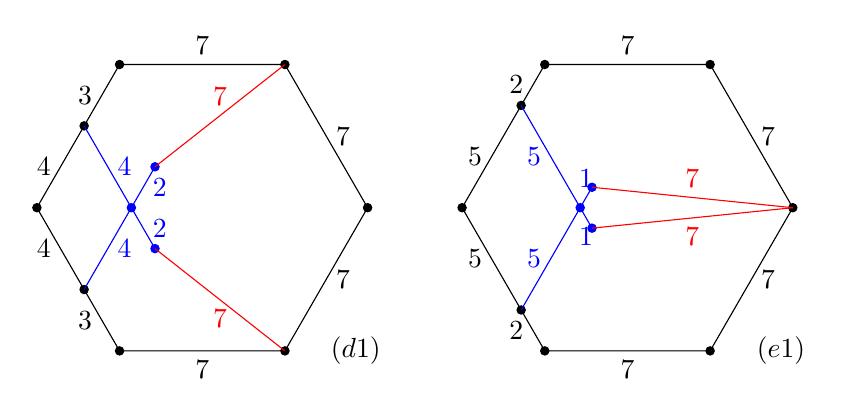
\begin{tikzpicture}
\def\x{0.5}
\def\y{0.866}
\begin{scope}[scale=0.3]

\begin{scope}[shift={(0,0)}] %row-1 col-1
\draw[black](10,0) node{$(d1)$};
\draw[black,fill=black](0,0)
 -- node[below] {7} ++(7,0) circle(5pt)
 -- node[right] {7} ++(7*\x,7*\y) circle(5pt)
 -- node[right] {7} ++(-7*\x,7*\y) circle(5pt)
 -- node[above] {7} ++(-7,0) circle(5pt)
 -- node[left] {3} ++(-3*\x,-3*\y) circle(5pt)
 -- node[left] {4} ++(-4*\x,-4*\y) circle(5pt)
 -- node[left] {4} ++(+4*\x,-4*\y) circle(5pt)
 -- node[left] {3} ++(3*\x, -3*\y) circle(5pt);
\draw[blue,fill=blue] (-3*\x,+3*\y)
 -- node[right] {4} ++(4*\x,4*\y) circle(5pt)
 -- node[right] {2} ++(2*\x,2*\y) circle(5pt)
 ++(0,-4*\y) circle(5pt)
 -- node[right] {2} ++(-2*\x,2*\y) circle(5pt)
 -- node[right] {4} ++(-4*\x,4*\y);
\draw[red] (3*\x,5*\y) -- node[below] {7} (7,0);
\draw[red] (3*\x,9*\y) -- node[above] {7} (7,14*\y);
\end{scope}

\begin{scope}[shift={(18,0)}] %row-1 col-2
\draw[black](10,0) node{$(e1)$};
\draw[black,fill=black](0,0)
 -- node[below] {7} ++(7,0) circle(5pt)
 -- node[right] {7} ++(7*\x,7*\y) circle(5pt)
 -- node[right] {7} ++(-7*\x,7*\y) circle(5pt)
 -- node[above] {7} ++(-7,0) circle(5pt)
 -- node[left] {2} ++(-2*\x,-2*\y) circle(5pt)
 -- node[left] {5} ++(-5*\x,-5*\y) circle(5pt)
 -- node[left] {5} ++(+5*\x,-5*\y) circle(5pt)
 -- node[left] {2} ++(2*\x, -2*\y) circle(5pt);
\draw[blue,fill=blue] (-2*\x,+2*\y)
 -- node[left] {5} ++(5*\x,5*\y) circle(5pt)
 -- node[above] {1} ++(1*\x,1*\y) circle(5pt)
 ++(0,-2*\y) circle(5pt)
 -- node[below] {1} ++(-1*\x,1*\y) circle(5pt)
 -- node[left] {5} ++(-5*\x,5*\y);
\draw[red] (4*\x,6*\y) -- node[below] {7} (7+7*\x,7*\y);
\draw[red] (4*\x,8*\y) -- node[above] {7} (7+7*\x,7*\y);
\end{scope}


\end{scope}
\end{tikzpicture}
\caption{
Variations of constructions of the nice hexagon side $a=7,b=1,e=7$.
Cases $(d1)$ and $(e1)$ are adaptations of cases $(d)$ and $(e)$ of figure \ref{fig:nice-hexagon} where only the blue strips are displaced. Such changes mantain the internal bolts,
red strips and perimeter the same. The original \textbf{Triple unit} $a,b,c,d,e$ irregular pentagon 
is replaced by an irregular hexagon clearly visible in case $(e1)$.
}
\label{fig:nice-hexagon-var}
\end{figure}

\newcommand{\nicehexagon}[5] %a,b,c,d,e
{
\def\x{0.5}
\def\y{0.866}
\pgfmathsetmacro{\ab}{int(#1-#2)} %a-b
\pgfmathsetmacro{\ac}{int(#1-#3)} %a-c
\pgfmathsetmacro{\bdA}{int(#4-#2)} %-b+d
\pgfmathsetmacro{\bdB}{int(#2+#4)} %b+d
\draw[black,fill=black](0,0)
 -- node[below]{#1} ++(#1,0) circle(5pt) %+a,0
 -- node[right]{#3} ++(#3*\x,#3*\y) circle(5pt) %cx,cy
 -- node[right]{\ac} ++(\ac*\x,\ac*\y) circle(5pt)
 -- node[right]{\ac} ++(-\ac*\x,\ac*\y) circle(5pt)
 -- node[right]{#3} ++(-#3*\x,#3*\y) circle(5pt)
 -- node[above]{#1} ++(-#1,0) circle(5pt) %-a,0
 -- node[left]{#2} ++(-#2*\x,-#2*\y) circle(5pt) %b
 -- node[left]{\ab} ++(-\ab*\x,-\ab*\y) circle(5pt) %a-b
 -- node[left]{\ab} ++(+\ab*\x,-\ab*\y) circle(5pt)
 -- node[left]{#2} ++(#2*\x, -#2*\y) circle(5pt);
\draw[blue] (-#2*\x,+#2*\y) %bx,by
 -- node[left]{\ab} ++(\ab*\x,\ab*\y) circle(5pt)
 -- node[left]{\ab} ++(-\ab*\x,\ab*\y);
\draw[red] (#1+#3*\x,#3*\y) %a+cx,cy
 -- node[below]{#5} (\bdA*\x,\bdB*\y) %(-b+d)x,(b+d)y
 -- node[above]{#5} (#1+#3*\x,#3*\y + 2*\ac*\y); %a+cx,(c+2(a-c))y
}

\begin{figure}[h]
\centering
\begin{tikzpicture}

\begin{scope}[scale=0.15]
\begin{scope}[shift={(0,0)}] %row-1 col-1
\nicehexagon{13}{2}{5}{11}{13}
\end{scope}
\begin{scope}[shift={(32,0)}] %row-1 col-2
\nicehexagon{14}{1}{6}{13}{13}
\end{scope}
\begin{scope}[shift={(66,0)}] %row-1 col-3
\nicehexagon{15}{1}{5}{14}{14}
\end{scope}
\begin{scope}[shift={(10,-44)}] %row-2 col-1
\nicehexagon{19}{2}{3}{17}{19}
\end{scope}
\begin{scope}[shift={(55,-44)}] %row-2 col-2
\nicehexagon{20}{1}{4}{19}{19}
\end{scope}
\end{scope}

\end{tikzpicture}
\caption{More nice hexagons from sizes $13 - 20$.}
\label{fig:nice-hexagon-more} 
\end{figure}

\section{Regular octagons}

We replace the cosines for octagon in table \ref{tbl:polygons} in $e^2$ equation:
\begin{align}
e^2 &= a^2 +b^2 +c^2 +d^2 -2(ab+ac+bd)\cos\theta +2(bc+ad)\cos(2\theta) -2cd\cos(3\theta) \nonumber\\
 &= a^2 +b^2 +c^2 +d^2 
 -2(ab+ac+bd)\left(-\frac{\sqrt{2}}{2}\right) 
 +2(bc+ad)\left(0\right) 
 -2cd\left(\frac{\sqrt{2}}{2}\right) \nonumber\\
 &= a^2 +b^2 +c^2 +d^2 +(ab +ac +bd -cd)\sqrt{2}
\end{align} 

$e$ cannot to be and integer if the factor of $\sqrt{2}$ is not zero, so we force this factor to be zero:
\begin{align*}
ab + ac + bd - cd &= 0 \\
a(b+c) &= (c-b)d \\
e^2 &= a^2 +b^2 +c^2 +d^2 + (0)\sqrt{2}
\end{align*}

\coloredeq{eq:octagon-e}{
e = \sqrt{a^2 +b^2 +c^2 +d^2 } \quad\Longleftrightarrow\quad a(b+c) &= (c-b)d
}


\subsection{Octagons examples}

\textbf{Conjecture}: No possible octagons formed with triple unit.

\section{Equilateral decagons}

We replace the cosines for decagon in table \ref{tbl:polygons} in $e^2$ equation:
\begin{align}
e^2 &= a^2 +b^2 +c^2 +d^2 -2(ab+ac+bd)\cos\theta +2(bc+ad)\cos(2\theta) -2cd\cos(3\theta) \nonumber\\
 &= a^2 +b^2 +c^2 +d^2
  -2(ab+ac+bd)\left(\dfrac{-1-\sqrt{5}}{4}\right)
  +2(bc+ad)\left(\dfrac{-1+\sqrt{5}}{4}\right)
  -2cd\left(\dfrac{-1+\sqrt{5}}{4}\right) \nonumber\\
 &= a^2 +b^2 +c^2 +d^2 +\frac{ab+ac+bd -bc-ad +cd}{2} +\frac{ab+ac+bd +bc+ad -cd}{2}\sqrt{5}
\end{align}
$e$ cannot to be and integer if the factor of $\sqrt{5}$ is not zero so we force this factor to be zero:
\begin{align}
 ab+ac+bd +bc+ad -cd &= 0\nonumber\\
 ab+ac+bd &= cd -bc-ad \\
 ab+ac+bc &= (c -a -b)d
\end{align}
We replace $ab+ac+bd$ by $cd -bc-ad$ in the $e^2$ equation to get:
\begin{align}
e^2 &= a^2 +b^2 +c^2 +d^2 +\frac{(cd -bc-ad) -bc-ad+cd}{2} +\frac{0}{2}\sqrt{5} \nonumber\\
 &= a^2 +b^2 +c^2 +d^2 + cd -bc -ad\nonumber
\end{align}

\coloredeq{eq:decagon-e}{
e = \sqrt{a^2 +b^2 +c^2 +d^2 -bc -(a-c)d } \quad\Longleftrightarrow\quad ab+ac+bc = (c -a -b)d
}

\subsection{Decagons software}

Common routine where $a \ge b,c$ doesn't return solutions. But when we change the condition $c \ge a$ we get 
other type of solutions.

\begin{lstlisting}
func TestDecagonsCBA(t *testing.T) {
    tri := NewTriples()
    tri.DecagonsCBA(500)
}

func (t *Triples) DecagonsCBA(max int) {
	for c := 1; c <= max; c++ {
		for b := 1; b <= c; b++ {
			for a := 1; a <= c; a++ {
				ab_ac_bc := a*b + a*c + b*c
				aa_bb_cc := a*a + b*b + c*c
				for d := 1; d <= max; d++ {
					if ab_ac_bc != (c-a-b)*d {
						continue // condition to reject sqrt{5} from e equation
					}
					if e, ok := t.squareRoot(aa_bb_cc + d*d - b*c -(a-c)*d); ok {
						t.Add(a, b, c, d, e)
					}
				}
			}
		}
	}
}
\end{lstlisting}

The software solutions are in next listing. As with the case for pentagons,
we \textbf{conjecture} again the variable $e$ is in the form $10x + 1, x \in \bbb{Z}$ or simply:
\begin{align}
e \equiv 1\mod{10}
\end{align}

\setlength{\columnsep}{50pt}
\begin{multicols}{2}
\begin{lstlisting}
  1  a=  8 b=  4 c= 13 d=188 e=191
  2  a=  3 b=  6 c= 18 d= 20 e= 31
  3  a=  6 b=  3 c= 20 d= 18 e= 31
  4  a= 12 b=  8 c= 36 d= 51 e= 71
  5  a= 24 b=  8 c= 51 d= 96 e=121
  6  a=  8 b= 12 c= 51 d= 36 e= 71
  7  a= 42 b=  7 c= 60 d=294 e=311
  8  a= 20 b= 30 c= 75 d=174 e=211
  9  a= 44 b= 24 c= 84 d=423 e=451
 10  a=  2 b= 63 c= 84 d=294 e=341
 11  a=  7 b= 57 c= 93 d=219 e=271
 12  a=  8 b= 24 c= 96 d= 51 e=121
 13  a= 60 b= 15 c=104 d=300 e=341
 14  a= 42 b= 36 c=114 d=289 e=341
 15  a= 45 b= 24 c=128 d=168 e=241
 16  a= 15 b= 57 c=133 d=171 e=251
 17  a= 72 b= 39 c=152 d=480 e=541
 18  a= 24 b= 84 c=153 d=412 e=491
 19  a= 13 b= 83 c=167 d=241 e=341
 20  a= 24 b= 45 c=168 d=128 e=241
 21  a= 53 b= 55 c=169 d=347 e=431
 22  a= 57 b= 15 c=171 d=133 e=251
 23  a= 21 b= 91 c=171 d=357 e=451
 24  a= 30 b= 20 c=174 d= 75 e=211
 25  a=  4 b=  8 c=188 d= 13 e=191
 26  a=117 b=  3 c=219 d=269 e=401
 27  a= 57 b=  7 c=219 d= 93 e=271
 28  a= 28 b= 98 c=221 d=322 e=451
 29  a= 34 b= 93 c=228 d=318 e=451
 30  a= 83 b= 13 c=241 d=167 e=341
 31  a=109 b= 24 c=264 d=288 e=451
 32  a= 24 b=144 c=267 d=488 e=641
 33  a=  3 b=117 c=269 d=219 e=401
 34  a= 36 b= 96 c=276 d=277 e=451
 35  a= 96 b= 36 c=277 d=276 e=451
 36  a= 24 b=109 c=288 d=264 e=451
 37  a= 36 b= 42 c=289 d=114 e=341
 38  a= 63 b=  2 c=294 d= 84 e=341
 39  a=  7 b= 42 c=294 d= 60 e=311
 40  a= 15 b= 60 c=300 d=104 e=341
 41  a= 93 b= 34 c=318 d=228 e=451
 42  a= 98 b= 28 c=322 d=221 e=451
 43  a= 55 b= 53 c=347 d=169 e=431
 44  a= 91 b= 21 c=357 d=171 e=451
 45  a=105 b= 87 c=363 d=461 e=671
 46  a=180 b= 24 c=380 d=465 e=691
 47  a=105 b= 90 c=406 d=420 e=671
 48  a= 84 b= 24 c=412 d=153 e=491
 49  a= 90 b=105 c=420 d=406 e=671
 50  a= 24 b= 44 c=423 d= 84 e=451
 51  a=222 b= 12 c=454 d=495 e=781
 52  a= 87 b=105 c=461 d=363 e=671
 53  a= 24 b=180 c=465 d=380 e=691
 54  a= 39 b= 72 c=480 d=152 e=541
 55  a=144 b= 24 c=488 d=267 e=641
 56  a= 12 b=222 c=495 d=454 e=781
--- PASS: TestDecagonsCBA (42.31s)
\end{lstlisting}
\end{multicols}

\subsection{Decagons examples}

\newcommand{\decagonTriple}[5] %a,b,c,d,e c>a, c>b
{
\pgfmathsetmacro{\ca}{int(#3-#1)} %c-a
\pgfmathsetmacro{\cb}{int(#3-#2)} %c-b
\pgfmathsetmacro{\bx}{#2*cos(36)}
\pgfmathsetmacro{\by}{#2*sin(36)}
\pgfmathsetmacro{\cx}{#3*cos(36)}
\pgfmathsetmacro{\cy}{#3*sin(36)}
\pgfmathsetmacro{\cxx}{#3*cos(72)}
\pgfmathsetmacro{\cyy}{#3*sin(72)}
\pgfmathsetmacro{\dxx}{#4*cos(72)}
\pgfmathsetmacro{\dyy}{#4*sin(72)}
\pgfmathsetmacro{\cax}{\ca*cos(36)}
\pgfmathsetmacro{\cay}{\ca*sin(36)}
\pgfmathsetmacro{\cbx}{\cb*cos(36)}
\pgfmathsetmacro{\cby}{\cb*sin(36)}
\pgfmathsetmacro{\ax}{#1*cos(36)}
\pgfmathsetmacro{\ay}{#1*sin(36)}
\coordinate(O) at (0,0);
\coordinate(B) at (#1,0);
\coordinate(C) at (#1+\cx, \cy);
\coordinate(D) at (#1+\cx+\cxx, \cy+\cyy);
\coordinate(H) at (-\bx,\by);
\coordinate(L) at (-\bx-\dxx,\by+\dyy);
\coordinate(A) at (-\ca,0);
\coordinate(AC) at (-\ca-\cax,+\cay);
\coordinate(J) at (-\ca-\cax-\ax, +\cay+\ay);
\coordinate(I) at (-\ca-\cax-\ax-\cxx, +\cay+\ay+\cyy);
\coordinate(II) at (-\cax-\ax-\cxx, +\cay+\ay+\cyy);
\coordinate(III) at (-\cax-\ax-\cxx+\cbx, +\cay+\ay+\cyy-\cby);
\coordinate(JJ) at (-\cax-\ax, +\cay+\ay);
\draw[red,fill=red](C) node[right]{$C$}
 -- node[above]{$#3$} (B) node[below]{$B$} circle(5pt) 
 -- node[above]{$#1$} (O) circle(5pt)
 -- node[above]{$#2$} (H) circle(5pt)
 -- node[right]{$#4$} (L) circle(5pt)
 -- node[below]{$#5$} (C) circle(5pt)
 ;
\draw[black,fill=black] (O) node[below]{$O$}
 -- node[below]{$\ca$} (A) node[below]{$A$} circle(5pt)
 -- node[below,red]{$#3$} (J) node[left]{$J$} circle(5pt)
 -- node[above]{$\ca$} (JJ) circle(5pt)
 -- node[above,blue]{$\cb$} (H) circle(5pt)
 (J)
 -- node[left,red]{$#3$} (I) node[left]{$I$} circle(5pt)
 -- node[above]{$\ca$} (II) circle(5pt)
 -- node[left,red]{$#3$} (JJ) circle(5pt)
 (II)
 -- node[above,blue]{$\cb$} (III) circle(5pt)
 -- (L)
 ;
\draw[black,fill=black](C) 
 -- node[right,red]{$#3$} (D) node[right]{$D$} circle(5pt)
 ;
}

\begin{figure}[H]
\centering
\begin{tikzpicture}
\begin{scope}[scale=0.12]
 \begin{scope}[shift={(0,0)}] %row-1 col-1
  \decagonTriple{3}{6}{18}{20}{31}
 \end{scope}
 \begin{scope}[shift={(70,0)}] %row-1 col-2
  \decagonTriple{6}{3}{20}{18}{31}
 \end{scope}
\end{scope}
\end{tikzpicture}
\caption{Half of decagons with $e=31$, sizes $18$ and $20$.}
\label{fig:decagons-31} 
\end{figure}

\begin{figure}[H]
\centering
\begin{tikzpicture}
\begin{scope}[scale=0.06]
 \begin{scope}[shift={(0,0)}] %row-1 col-1
  \decagonTriple{12}{8}{36}{51}{71}
 \end{scope}
 \begin{scope}[shift={(0,-90)}] %row-2 col-1
  \decagonTriple{8}{12}{51}{36}{71}
 \end{scope}
\end{scope}
\end{tikzpicture}
\caption{Half of decagons with $e=71$, sizes $36$ and $51$.}
\label{fig:decagons-71} 
\end{figure}


\begin{figure}[H]
\centering
\begin{tikzpicture}
\begin{scope}[scale=0.04]
 \begin{scope}[shift={(0,0)}] %row-1 col-1
  \decagonTriple{24}{8}{51}{96}{121}
 \end{scope}
 \begin{scope}[shift={(0,-160)}] %row-2 col-1
  \decagonTriple{8}{24}{96}{51}{121}
 \end{scope}
\end{scope}
\end{tikzpicture}
\caption{Half of decagons with $e=121$, sizes $51$ and $96$.}
\label{fig:decagons-121} 
\end{figure}

With the results where $c > a$ we need to add helping rhombi to start
building complete decagons. See figures \ref{fig:decagons-31},
\ref{fig:decagons-71} and \ref{fig:decagons-121}. In red we have the unit, for each
pair for the same $e$ the pairs interchage segments $a,b$ and $c,d$. The complete
building and dispositions of helping strips and rigidity is beyond this paper.





\end{document}